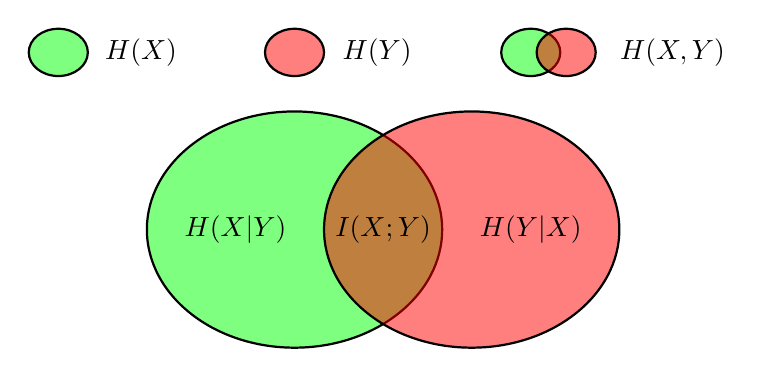
\begin{tikzpicture}[thick, scale=1.5]
    \draw [fill opacity=0.5,fill=green] (1,1) ellipse (1.25 and 1);
    \draw [fill opacity=0.5,fill=red] (2.5,1) ellipse (1.25 and 1);
    
    \draw [fill opacity=0.5,fill=green] (-1,2.5) ellipse (1.25*0.2 and 1*0.2);
    \node at (-0.3,2.5) {$H(X)$};

    \draw [fill opacity=0.5,fill=red] (-1+2,2.5) ellipse (1.25*0.2 and 1*0.2);
    \node at (-0.3+2,2.5) {$H(Y)$};

    \draw [fill opacity=0.5,fill=green] (-1+4,2.5) ellipse (1.25*0.2 and 1*0.2);
    \draw [fill opacity=0.5,fill=red] (-1+4+1.5*0.2,2.5) ellipse (1.25*0.2 and 1*0.2);
    \node at (0.2+4,2.5) {$H(X,Y)$};

    \node at (1.75,1) {$I(X;Y)$};
    \node at (0.5,1) {$H(X|Y)$};
    \node at (3,1) {$H(Y|X)$};
\end{tikzpicture}